\chapter{Expected findings and schedule of work}
Developing a design procedure that provides resilient bridges is one of the main goals of this study.This research will develop a displacement based design tool, that achieves that goal. This chapter introduces the overall design concept, then the direct displacement based design (DDBD) is presented and a proposed modifications to this design methodology, based on corroded RC physical tests results, are shown. Finally a schedule of work is presented.

\section{Condition dependent performance based design concept}

Current design methodologies in earthquake engineering follow the performance based design philosophy. This methodology has allowed engineers and stake holders of infrastructure projects to design and build structures that will achieve a performance goal during the service life of the structure. Implied in this methodology is the assumption that the properties of the structure will remain unchanged, that is the structure will maintain it's pristine conditions properties. We know by observing existing structures in our environment, that structures age, and from the information presented in the previous chapters, it is possible to account for this aging to design resilient structures. Figure \ref{fig:Concept_CD-DDBD} schematically shows what would happen to structures designed to pristine conditions as it ages. Essentially, current designs would render a structure close to damage limit states if left alone, sooner than the assumed service life. On the other hand our design approach while it won't eliminate aging, aims to allow structures to remain well above a prescribed limit state before the structure reaches the end of it's service life. 

\begin{figure}[htbp]
	\centering
	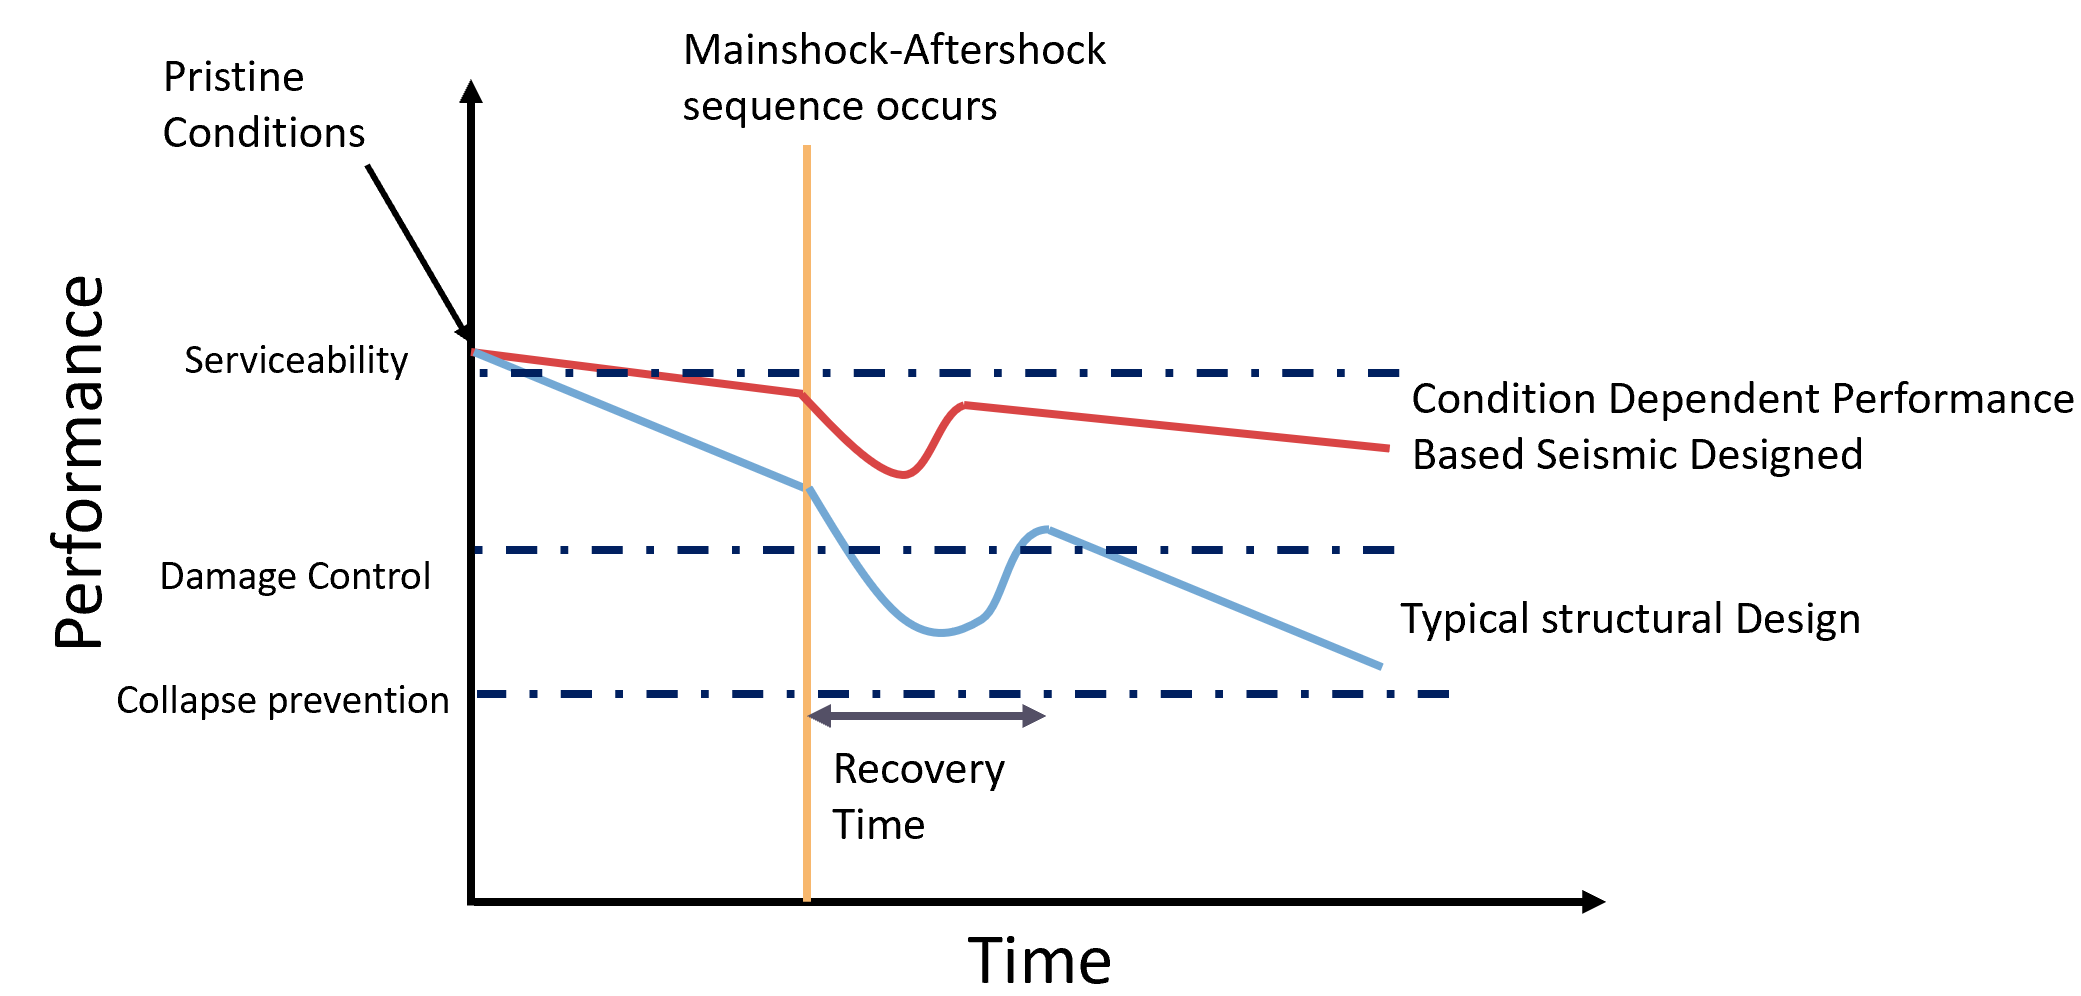
\includegraphics[width=0.90\textwidth]{VAC Prelim 2.0/Chapter-5/figs/CD_DDBD_Concept.png}
	\caption{Schematic concept of condition dependent performance based design and traditional designs}
	\label{fig:Concept_CD-DDBD}
\end{figure}

One of the design procedures in performance  based design is the direct displacement based design methodology. This research will modify components of the DDBD procedure to account for aging of the structures. The following sections present a summary on the DDBD methodology, as well as proposed components of the DDBD methodology that could be modified to incorporate our findings.

\section{Condition dependent direct displacement based design (CD-DDBD)}
\subsection{Overview of direct displacement based design}

While direct displacement based design (DDBD) is a well known procedure (see \cite{Priestley2007}), an overview of the methodology is presented here for convenience for a SDOF system. DDBD consists of five fundamental steps 1) characterize the limit states of the structure, these limit states correspond to structural damage or prescribed maximum drifts. For instance, in corroded RC circular columns, buckling of the corroded reinforcement is a limit state that precedes the strength degradation of the system. These limit states are then used to calculate the target displacements for the design. The goal of DDBD it to ensure that the structure reaches a desired performance by reaching the target displacement, for a given displacement spectra.  2) The equivalent viscous damping ($\xi_e$) is calculated using equations developed for different structural systems. Equivalent viscous damping depends on the expected ductility at the target displacement, and the force displacement hysteresis shape of the structural system ($\xi_{hyst}$), for example a modernly detailed RC structure will have a "fatter" hysteresis shape than an older structures. 3)  the effective period ($T_e$) of the structure is determined by entering with the target displacement ($\Delta_d$) and intersecting the design displacement spectra at the level of damping found in step (2) . The effective period is  the period of the structure at peak response. 4) The effective stiffness is calculated using the dynamic properties of the equivalent structure, plugging in the values in $K_e=\frac{4\pi^{2}m_{e}}{T_{e}}$. 5) Finally, The base shear is calculated using the stiffness equation, calculated as $V_{be}=K_{e}\Delta_{d}$.

\begin{figure}[htbp]
	\centering
	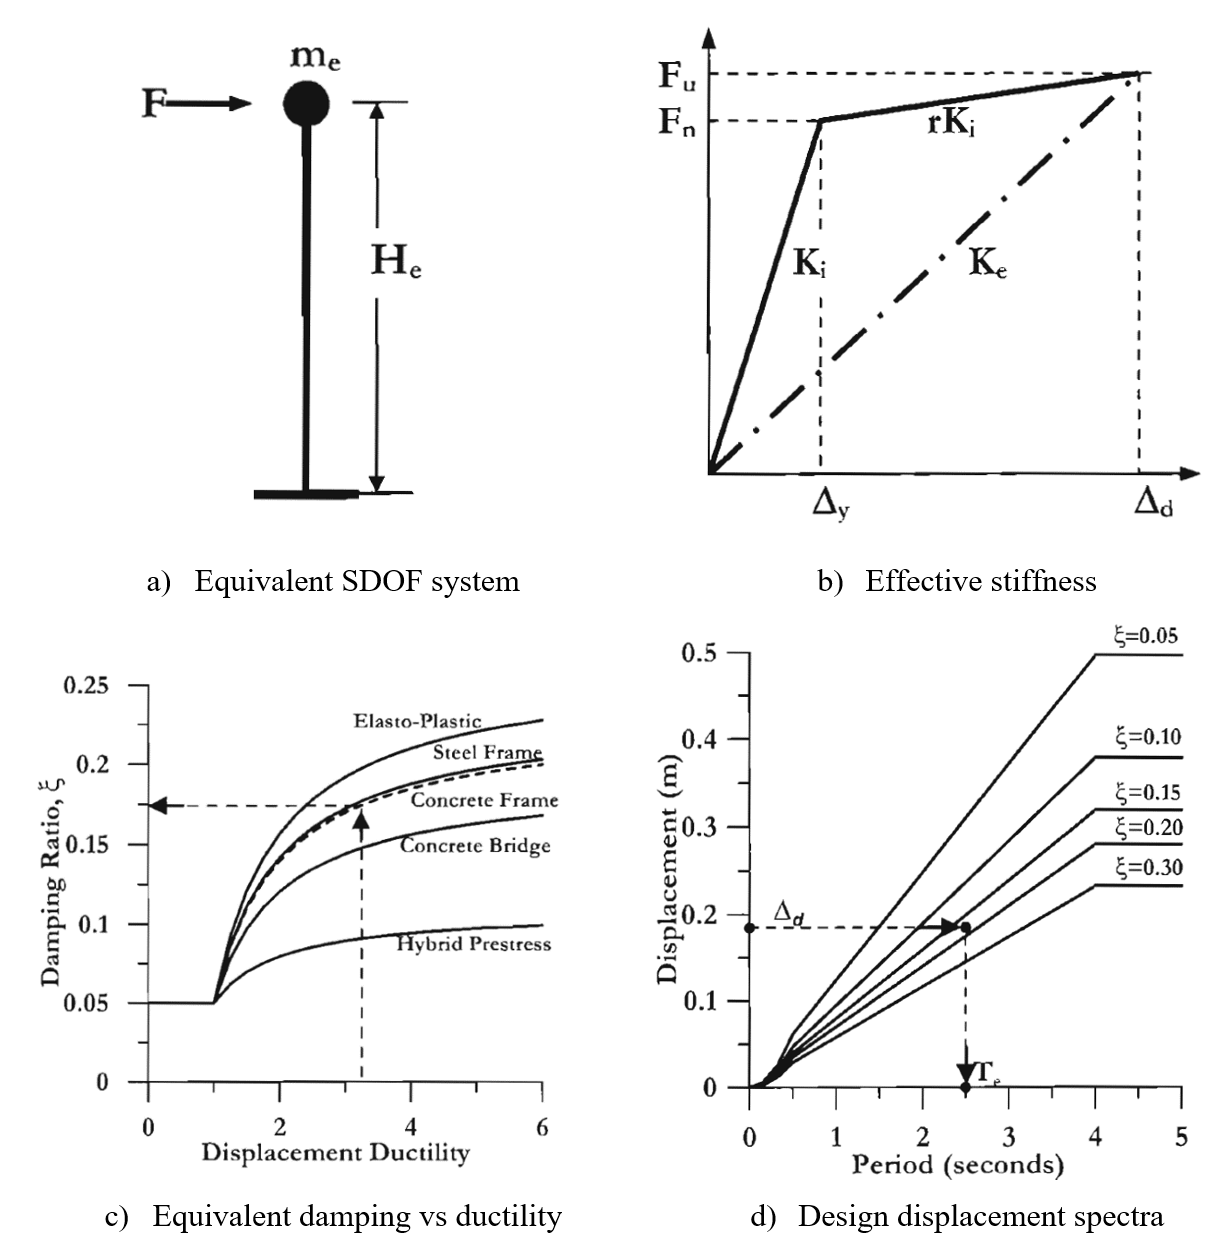
\includegraphics[width=0.75\textwidth]{VAC Prelim 2.0/Chapter-5/figs/DDBD.png}
	\caption{Direct displacement based design method summary \cite{Priestley2007}}
	\label{fig:DDBD_sum}
\end{figure}
\newpage

\subsection{Proposed design methodology}

Recent studies conducted in corroded RC columns have shown that the performance of these systems is greatly decreased the corrosion. These studies have shown that corroded structures have a lower strength, and displacement capacity as shown below. We hypothesize that the hysteresis area of the force displacement is lower in the corroded RC structure when compared to its pristine counterpart. For the DDBD procedure, this implies that the equivalent damping component follows the same trend. An analysis of the results of corroded structure is further expanded in this section. 

\textbf{Jacobsen damping in corroded RC structure physical tests.}

Figure \ref{fig:MedaJacobsen} shows teh force-displacement relationship from corred, and pristine condtion RC structures from a study performed by Meda et al \cite{Meda2014}. Jacobse damping used to to quantify the hysteretic damping, defined as shown in \eref{eq:JacobsenEquation}. For these structures, $\xi_{CL=0}=31.4\%$, and for the corroded structure $\xi_{CL=0}=24.2\%$, which corresponds to a reduction of $23\%$. Performing the same analysis to the results from a similar study from Ma et al \cite{Ma2012} a simmilar trend is observed.

\begin{equation}
    \xi=\frac{A_h}{2*\pi*F_m*\Delta_m}
    \label{eq:JacobsenEquation}
\end{equation}

Plotting the Jacobsen damping for these tests in function of the corrosion level (CL), and the level of axial load ratio ($ALR=\frac{P}{A_{g}f'_{c}}$), shown in \fref{fig:JacobsenResults}. Our analysis of these studies show that as the corrosion level, and the axial load ratio in the columns increases, the hysteretic damping decreases. While the scope of their studies were limited, due to non modern detailing used, and the accelerated corrosion process used high levels of current density, they provide an insight at the consequences of corrosion. 

\begin{figure}[htbp]
	\centering
    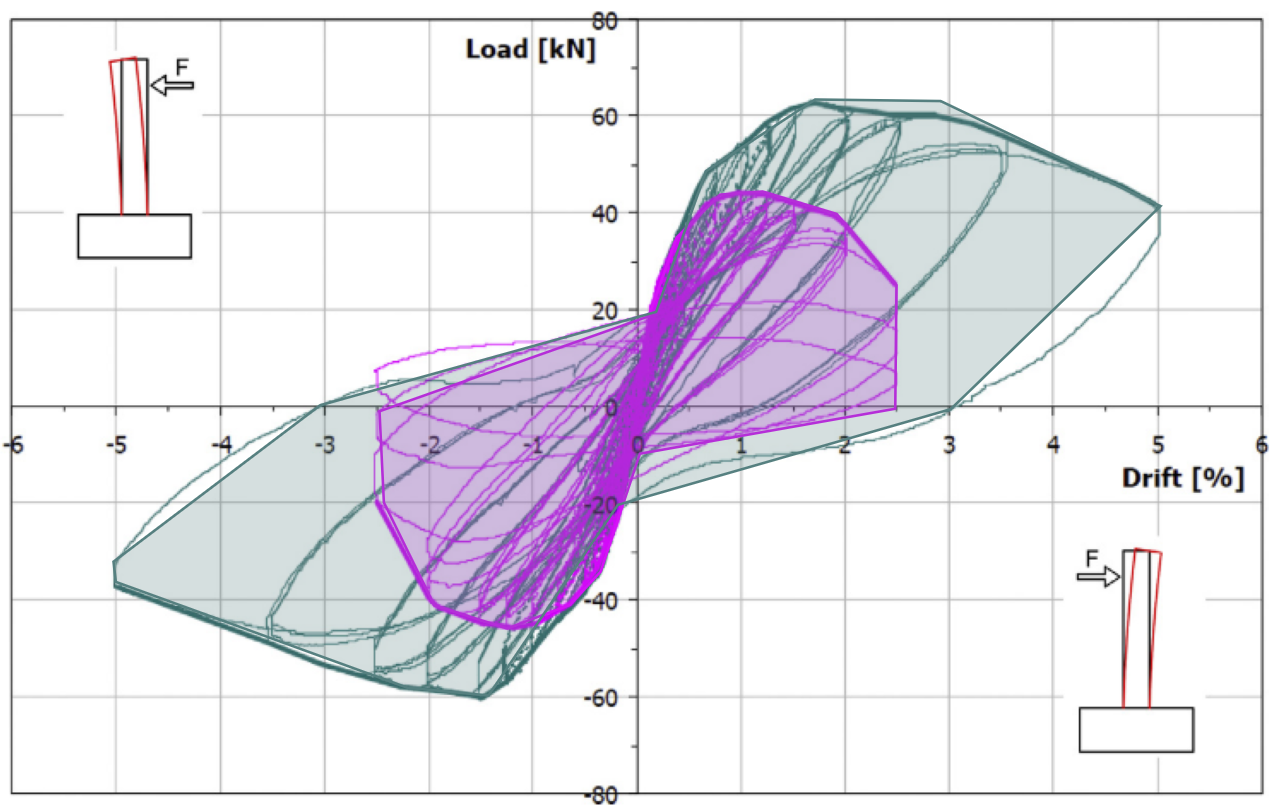
\includegraphics[width=0.75\textwidth]{VAC Prelim 2.0/Chapter-5/figs/Meda_HystereticArea_01.png}
	\caption{Hysteretic energy dissipation in pristine and corroded RC from Meda et al \cite{Meda2014}}
	\label{fig:MedaJacobsen}
\end{figure}

\begin{figure}[htbp]
	\centering
    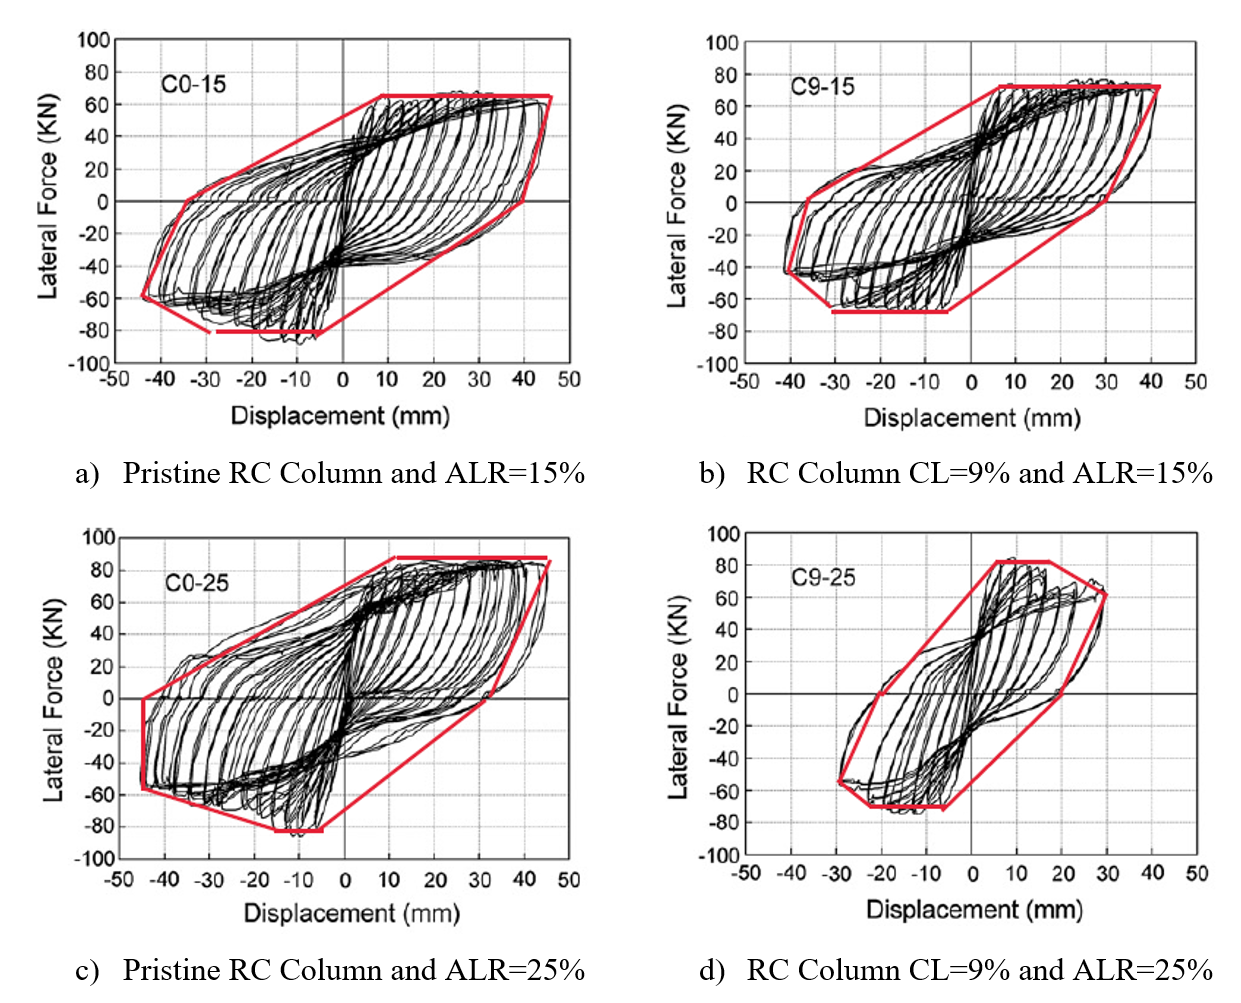
\includegraphics[width=0.75\textwidth]{VAC Prelim 2.0/Chapter-5/figs/Ma_HystereticArea_01.png}
	\caption{Hysteretic energy dissipation in pristine and corroded RC from Ma et al \cite{Meda2014}}
	\label{fig:MaJacobsen}
\end{figure}

\begin{figure}[htbp]
	\centering
    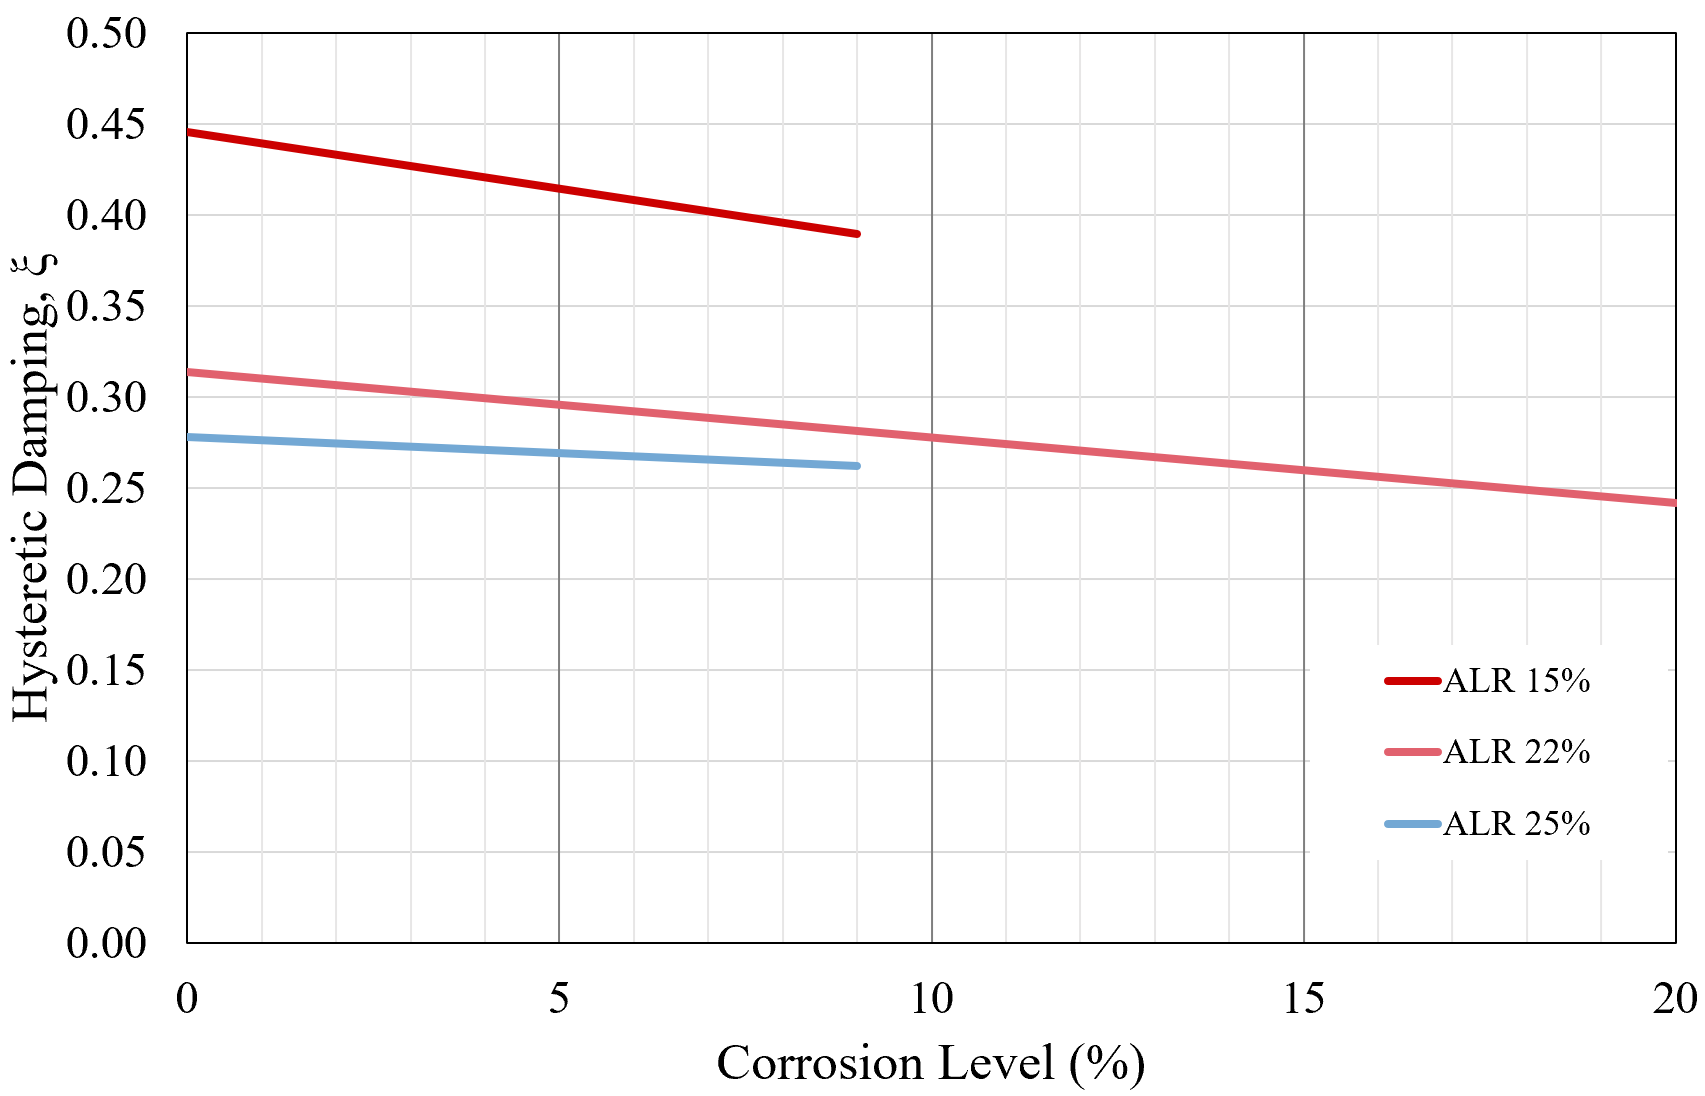
\includegraphics[width=0.75\textwidth]{VAC Prelim 2.0/Chapter-5/figs/HystereticDampingLitResults.png}
	\caption{Jacobsen hysteretic damping from Ma et al \cite{Ma2012}, and Meda et al \cite{Meda2014}}
	\label{fig:JacobsenResults}
\end{figure}

\textbf{Proposed changes DDBD}

Corrosion greatly impacts the hysteretic damping of corroded RC structures, and changes in the limit states of corroded rebars as a results of the epxerimental program outcomes. Furthermore in some cases the design could be controlled by shear due to the deterioration of the entire system. Therefore, we are proposing to include the effects of aging in two different inputs in DDBD by changing 1) The design displacement is calculated using the limit states that relate to corrosion, and 2) the equations used to determine the equivalent damping can be modified with a factor that relates to corrosion.

\section{Schedule of work}